\chapter{Sonde de température}
\label{chap:temperature_sensor}
Le capteur QCM intègre une sonde de température juste en dessous du quartz. Cependant, après avoir fait plusieurs tests avec un thermomètre, nous avons constaté que la mesure de température fournie par le capteur n'était pas toujours fiable. Des écarts de température allant jusqu'à 5 degrés Celsius ont été observés entre les deux capteurs.
Pour remédier à ce problème, il a été décidé d’automatiser la prise de température et d’ajouter la possibilité d’utiliser un capteur de température externe, pouvant être placé directement dans le liquide en utilisant la cellule électrochimique

\section{Choix du capteur de température}

\begin{table}[H]
\centering
\begin{tabularx}{\textwidth}{|l|X|X|X|}
\hline
\textbf{Critère}      & \textbf{Thermistance (NTC)} & \textbf{Thermocouple (Type K)} & \textbf{RTD (Pt100)} \\
\hline
Précision             & 2 & 1 & 3 \\
Linéarité             & 1 & 2 & 3 \\
Temps de réponse      & 2 & 3 & 1 \\
Plage (°C)            & 1 & 3 & 2 \\
Coût                  & 3 & 2 & 1 \\
Disponibilité         & 2 & 1 & 3 \\
\hline
Total                 & 11 & 12 & 13 \\
\hline
\end{tabularx}
\caption{Comparaison des capteurs thermiques (notation de 1 à 3, 3 étant le meilleur)}
\end{table}

Le choix s'est porté sur le capteur PT100 principalement pour sa précision et sa linéarité, ce qui rend le programme d'interprétation des données plus simple.

\section{Conditionnement du signal}
Le capteur PT100 nécessite un conditionnement du signal pour convertir la variation de résistance en une tension mesurable.
Le circuit de conditionnement est composé d'un pont de Wheatstone, d'un amplificateur de tension, d'un filtre passe-bas. Un microcontrôleur est ensuite utilisé pour convertir le signal analogique en numérique. Le microcontrôleur transmet également les données de température à l'ordinateur.

\fig[H, width=12cm]{Schéma du circuit de conditionnement pour la mesure de température avec la PT100}{ShemaElec.drawio}

\subsection{Pont de Wheatstone}
Le pont de Wheatstone est un circuit utilisé pour mesurer très précisément la variation de résistance de la sonde en fonction de la température. 
Il fonctionne en comparant la PT100 à des résistances de référence dans un montage équilibré. Toute variation de température modifie la résistance de la PT100, 
créant un déséquilibre mesurable sous forme de tension. Cette tension différentielle est proportionnelle à la variation de température.

\subsection{Amplificateur de tension}
L'amplificateur de tension est composé d'un amplificateur opérationnel et d'une résistance de gain. 
Il est utilisé pour amplifier le signal de tension issu du pont de Wheatstone.
L'amplification est nécessaire pour rendre le signal suffisamment fort pour être traité par le microcontrôleur.
L'amplificateur est configuré en mode non inverseur pour garantir que le signal reste positif et proportionnel à la variation de température.
Le gain de l'amplificateur est ajusté pour correspondre à la plage de tension acceptable par le microcontrôleur, à savoir entre 0 et 5V.

\subsection{Filtre passe-bas}
Lors des premiers tests de mesures de température avec la sonde PT100, il a été constaté que le signal de température était instable.
Chaque harmonique à laquelle le QCM vibrait donnait une température différente ; pour une harmonique donnée, la température restait stable (Figure~\ref{fig:TempBruit}).
\begin{figure}[H]
    \centering
    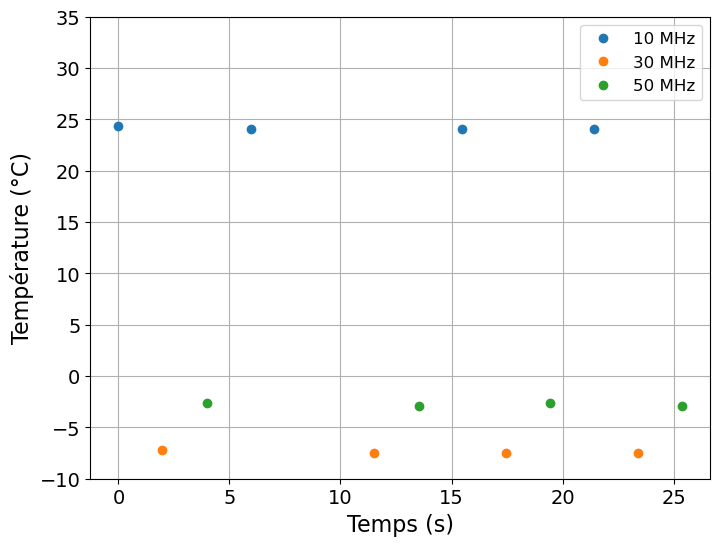
\includegraphics[width=0.8\textwidth]{assets/figures/TempBruit.png}
    \caption{Mesure de température avec perturbations}
    \label{fig:TempBruit}
\end{figure}

Plusieurs pistes ont été envisagées comme cause de ce problème : la sonde qui ne serait pas correctement isolée, une alimentation instable, ou encore des interférences électromagnétiques.
Les deux premières pistes ont été rapidement écartées, car la sonde est correctement isolée et l'alimentation est stable.
Pour vérifier notre troisième hypothèse, un oscilloscope a été utilisé pour observer le signal de sortie du pont de Wheatstone.

\begin{figure}[H]
    \centering
    \begin{minipage}{0.48\textwidth}
        \small
        Lors de la première harmonique, le signal à la sortie du pont de Wheatstone est bruité. 
        Sur la figure~\ref{fig:10mhzbruit}, on peut visualiser un signal oscillatoire d'une amplitude de 8,55\,mV et une longueur d'onde de 32\,ns, ce qui représente une fréquence de 31,25\,MHz.
        Cette fréquence est similaire à celle de la 3\textsuperscript{ème} harmonique du quartz de 10\,MHz, ce qui pourrait provenir d'un mode de résonance du quartz auquel il est spécialement sensible.
        Il est aussi intéressant de noter que l'amplitude est la plus petite des trois mesures et que la forme de l'onde n'est pas une sinusoïde contrairement aux deux autres.
    \end{minipage}\hfill
    \begin{minipage}{0.48\textwidth}
        \centering
        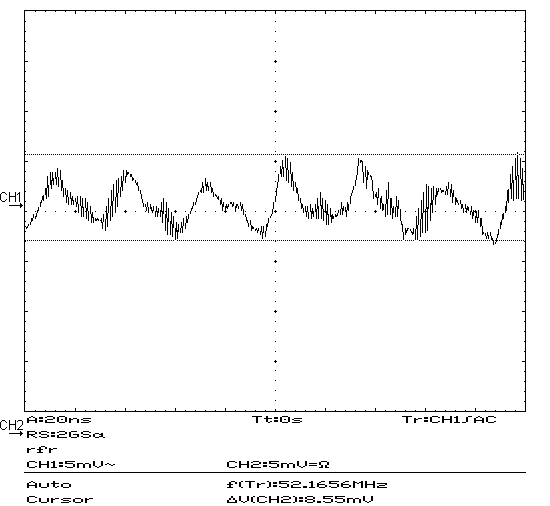
\includegraphics[width=\textwidth]{assets/figures/SCR00006.png}
        \caption{Vue de l'oscilloscope lors de l'excitation du quartz à 10MHz}
        \label{fig:10mhzbruit}
    \end{minipage}
\end{figure}

\begin{figure}[H]
    \centering
    \begin{minipage}{0.48\textwidth}
        \small
        Lors de la deuxième mesure avec un signal d'excitation de 30\,MHz, le signal à la sortie du pont de Wheatstone a une forme sinusoïdale avec une amplitude de 21\,mV, soit plus de deux fois le signal de la première mesure, et une longueur d'onde de 32\,ns, ce qui représente une fréquence de 31,25\,MHz.
        Cette fréquence est très similaire à la fréquence d'excitation du quartz.
    \end{minipage}\hfill
    \begin{minipage}{0.48\textwidth}
        \centering
        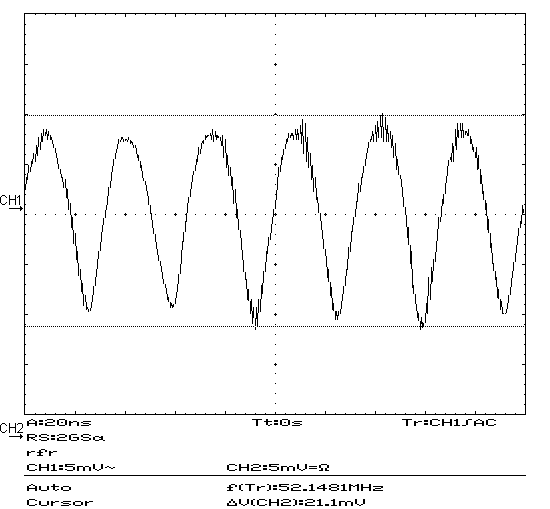
\includegraphics[width=\textwidth]{assets/figures/SCR00007.png}
        \caption{Vue de l'oscilloscope lors de l'excitation du quartz à 30MHz}
        \label{fig:30mhzbruit}
    \end{minipage}
\end{figure}

\begin{figure}[H]
    \centering
    \begin{minipage}{0.48\textwidth}
        \small
        Lors de la troisième mesure avec un signal d'excitation de 50\,MHz, le signal à la sortie du pont de Wheatstone a une forme sinusoïdale avec une amplitude de 18\,mV.
        La longueur d'onde est de 20\,ns, ce qui représente une fréquence de 50\,MHz, correspondant à la fréquence d'excitation du quartz.
    \end{minipage}\hfill
    \begin{minipage}{0.48\textwidth}
        \centering
        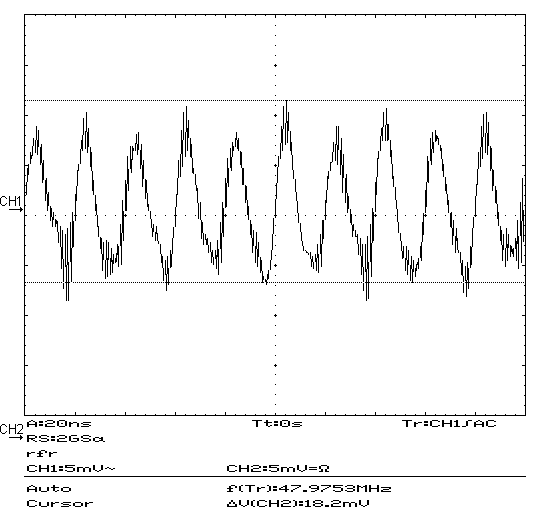
\includegraphics[width=\textwidth]{assets/figures/SCR00008.png}
        \caption{Vue de l'oscilloscope lors de l'excitation du quartz à 50MHz}
        \label{fig:50mhzbruit}
    \end{minipage}
\end{figure}

Une corrélation entre l'amplitude du signal mesurée et les perturbations de mesures de température de la figure \ref{fig:TempBruit} a été établie.
Cette perturbation est principalement due à la bande passante limitée de l'amplificateur opérationnel utilisé dans le circuit de conditionnement. Lorsque la fréquence du signal dépasse la bande passante de l'amplificateur, celui-ci n'est plus capable de suivre correctement les variations rapides, ce qui introduit du bruit et des distorsions dans la mesure de température.

Pour remédier à ce problème, un filtre passe-bas a été ajouté au circuit de conditionnement du signal.
Le filtre passe-bas est conçu pour atténuer les fréquences supérieures à 1 kHz, ce qui permet de réduire les interférences et de stabiliser la mesure de température.

Pour déterminer la fréquence de coupure du filtre passe-bas, on utilise la formule classique reliant la résistance $R$ et la capacité $C$ du filtre RC :

\begin{equation}
f_c = \frac{1}{2\pi RC}
\label{eq:frequence_coupure}
\end{equation}

où
\begin{itemize}
    \item $f_c$ est la fréquence de coupure en Hz,
    \item $R$ est la résistance en $\Omega$,
    \item $C$ est la capacité en $\mathrm{F}$.
\end{itemize}

Après avoir implémenté le filtre passe-bas, les mesures de température ont de nouveau été effectuées, dans les mêmes conditions que précédemment, c'est-à-dire dans l'eau distillée avec le capteur de température qui touche la surface du quartz pour avoir le maximum de perturbation.

\begin{figure}[H]
    \centering
    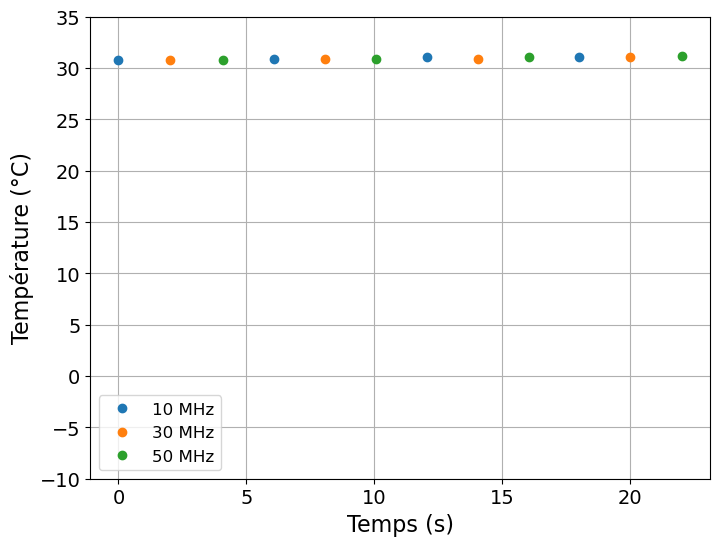
\includegraphics[width=0.8\textwidth]{assets/figures/TempFiltered.png}
    \caption{Mesure de température après application du filtre passe-bas}
    \label{fig:TempBruitFiltre}
\end{figure}

Les résultats sont excellents et la température est stable et ne varie pas de plus de 0,1°C entre les différentes harmoniques.
Le filtre passe-bas a donc permis de stabiliser la mesure de température en éliminant les perturbations dues aux fréquences indésirables.

\subsection{Calibration du capteur}
Une calibration est nécessaire pour connaître la conversion entre la tension en sortie du circuit et la température.
Pour ce faire, un étalonnage en utilisant un thermomètre de référence a été réalisé. La tension en sortie du circuit a été mesurée à différentes températures connues, permettant ainsi de calculer la relation entre la tension et la température, qui est linéaire dans le cas de la PT100.

\begin{figure}[H]
    \centering
    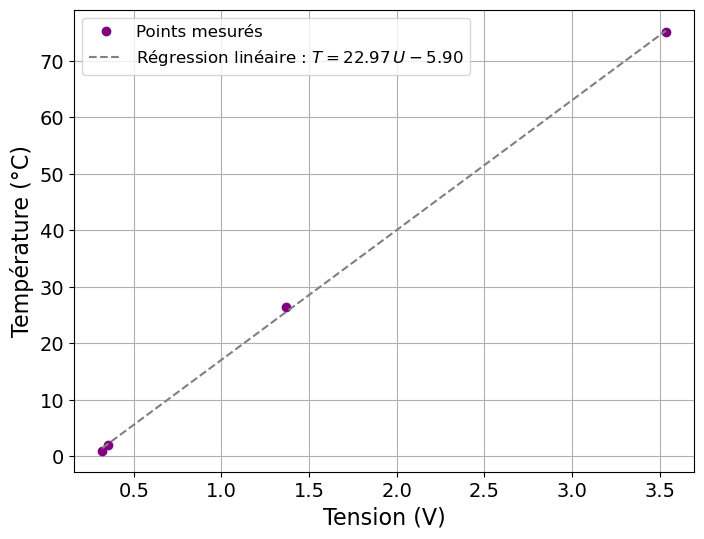
\includegraphics[width=0.8\textwidth]{assets/figures/CalibrationPT100.png}
    \caption{Calibration du capteur PT100}
    \label{fig:CalibrationPT100}
\end{figure}


